
\subsection{Real data: protein signalling}\label{sec:exp-sachs}

Every result so far comes from a simulation whose generating model is the one
the certificates assume. We therefore ran CERT-CD on the single-cell
protein-signalling data of \citet{sachs2005causal}, using the observational
condition only---$853$ cells, $11$ phosphoproteins, in the continuous form
distributed with \texttt{bnlearn} \citep{scutari2010learning}. Measurements
are log-transformed, as in the original analysis, since the raw fluorescence
intensities span three orders of magnitude and are strongly right-skewed. The
interventional conditions that make the Sachs network identifiable are
withheld, which makes this the hardest honest setting for a purely
observational method. We compare against the published $17$-arc consensus
network, and we stress that this is a scientific consensus assembled from
interventional experiments and prior literature, not ground truth; several of
its arcs are contested.

At $\alpha = 0.1$ and $k = 2$, streaming in batches of $50$ after a
$100$-observation warm-up that is discarded---so the e-processes see $753$
of the $853$ cells---CERT-CD certifies
$6$ edges out of $55$ pairs and leaves $49$ undecided. The two halves of the
output behave very differently, and the contrast is the reason to report the
experiment.

\paragraph{The adjacency half does what it claims.} All $6$ certified edges
lie in the consensus skeleton, and none outside it: Raf--Mek, PIP2--PIP3,
Erk--Akt, Akt--PKA, PKC--P38 and PKC--Jnk. Six of $17$ consensus edges is low
recall, which is what one expects from the $753$ observations the
certificates actually consume, a family-wise
budget over $55$ pairs, and a certificate that must reject to assert. PC at
the same level and order returns $7$ edges, all also in the consensus
skeleton, and then \emph{calls the remaining $48$ pairs absent}---an assertion
about $48$ pairs that this sample cannot support, and the one CERT-CD declines
to make. The difference between the two outputs is not the $6$ versus $7$
edges; it is the $49$ pairs one of them describes accurately.

\paragraph{The orientation half is confidently wrong.} All $4$ certified
arrowheads are reversed relative to the consensus: the certificate reports
Mek $\to$ Raf, PIP2 $\to$ PIP3, Akt $\to$ Erk and P38 $\to$ PKC, against
consensus arcs running the other way. Four out of four is not sampling
variation, and we investigated it rather than reporting it as an anomaly.

The reversal is a property of these data under a linear non-Gaussian model,
not of an idiosyncrasy of the sequential machinery. DirectLiNGAM produces a
causal order that reverses \emph{the same four arcs} (and agrees with the
consensus on Akt--PKA and PKC--Jnk, which the certificate left unoriented).
We do not read this agreement as independent corroboration: DirectLiNGAM uses
exactly the pairwise comparison of Eq.~\eqref{eq:direction}'s two branches
(Section~\ref{sec:related}), so the two procedures share their statistic and
their model, and agreeing on all four reversals is what two implementations
of the same comparison should do when the shared model is wrong, not evidence
that anything beyond the model has been ruled out. What the agreement does
show is that the reversal is not an artefact of the sequential
apparatus---the plain comparison reverses the same arcs with no e-process, no
threshold and no monitoring involved. The pairs in question are embedded in a
densely confounded, demonstrably nonlinear signalling network, where the
bivariate linear non-Gaussian model of Section~\ref{sec:direction} is simply
false. Under misspecification the supremum in~\eqref{eq:direction} is taken
over a model not containing the truth, and Proposition~\ref{prop:direction}
gives nothing (Remark~\ref{rem:misspec}).

We draw two conclusions and resist a third. First, the experiment is a clean
illustration of the asymmetry the paper is about: the certificate whose null
requires only the Markov condition behaves exactly as advertised on real data,
while the certificate whose null requires a parametric functional model fails
exactly where that model fails. Second, it shows that the failure is not
detectable from the output---the reversed arrowheads carry the same
$\alpha = 0.1$ label as any other, which is precisely why
Remark~\ref{rem:misspec} names misspecification as the construction's main
theoretical risk rather than a footnote. The conclusion we resist is that the
consensus is wrong and the certificates are right; observational
non-Gaussianity-based orientation disagreeing with interventional evidence is
much more likely to be the model failing than the biology.
Figure~\ref{fig:exp10} shows how slowly the certified set accumulates.

\paragraph{Against a 2026 comparator on the same data.} \citet{uehara2026iterative}
evaluates the same observational Sachs recording ($n=853$, $11$ proteins) and
reports, at a default operating point, direction precision $0.933$ and recall
$0.700$ against $21$ practitioner queries, with a cheaper $8$-query
configuration reaching precision and recall $1.000$. Three differences make
this a comparison of methods rather than a scoreboard. First, that protocol
is \emph{interactive}: it consumes expert answers to structural queries as
part of reaching its numbers, where CERT-CD uses none---an interactive method
that may ask a human is not doing the same task as one that may not, and a
higher precision bought with $21$ queries is not a free improvement over one
bought with zero. Second, its reference network has $20$ directed edges
including a PKA$\leftrightarrow$PIP3 feedback pair, not the $17$-arc acyclic
consensus of \citet{sachs2005causal} we certify against; a certificate-only
method built on a DAG cannot certify a cycle, so the two evaluations are
scored against different ground truths by construction, not by oversight.
Third, recall is a well-posed quantity for a method that outputs a complete
DAG at every operating point; for CERT-CD, at $\alpha=0.1$ recall over the
full $20$- or $17$-edge network is $6/17 \approx 0.35$ on the adjacency side
and $0/17$ on the (wrong) orientation side, and neither number means what
Uehara's recall means, since the undecided $49$ pairs are not a rejection.
We report the juxtaposition because it is the only case in this paper where a
comparator we already cite for other reasons evaluates the identical real
sample, not because the numbers settle anything against each other.

\subsection{A real bivariate direction benchmark}\label{sec:exp-tuebingen}

Sachs is one dataset. A single real instance, however carefully analysed,
cannot say whether Section~\ref{sec:exp-sachs}'s failure is characteristic of
the direction certificate on real data or a property of that one confounded,
nonlinear network. The standard corrective in the bivariate-direction
literature is the Tübingen cause-effect pairs benchmark
\citep{mooij2016distinguishing}: $108$ real pairs drawn from $37$ underlying
datasets across meteorology, biology, medicine, engineering and economics,
each with a direction the literature treats as ground truth---though, as the
benchmark's own documentation states and we repeat rather than launder, that
ground truth was not established by intervention. It is the benchmark
LiNGAM, ANM, IGCI and RECI are conventionally scored against, and, as far as
we can establish from the papers themselves, at least two of the 2025--2026
papers already cited in Section~\ref{sec:related} for other reasons evaluate
on it: \citet{ding2025gaussdetect} and the statistical-power diagnostic of
\citet{prakash2026power}. Six of the $108$ pairs have a multivariate cause or
effect and are excluded, matching standard practice for this benchmark's
bivariate accuracy figures; the excluded pair numbers are reported alongside
the result rather than silently dropped.

Running the direction certificate on each of the remaining $102$ pairs as an
unconditioned bivariate test (Eqs.~\eqref{eq:fwd}--\eqref{eq:bwd} with $Z$ an
intercept only), at $\alpha=0.1$: it certifies a direction for $14$ of $102$
pairs, a coverage of $0.137$. Coverage this low is itself informative---most
of these pairs are close to linear only locally, or their noise is not well
approximated by the generalised-Gaussian family of Eq.~\eqref{eq:gg}, and the
certificate's response to a poor fit is to stay silent, exactly as
Remark~\ref{rem:misspec} says it should. What the low coverage does not buy is
accuracy on the pairs where it does commit: of the $14$ certified pairs, $6$
agree with the benchmark's assumed ground truth, a weighted accuracy of
$0.557$, with a $95\%$ Wilson interval of $[0.214, 0.674]$ that comfortably
contains chance. The forced-choice comparison statistic---the same pairwise
likelihood ratio DirectLiNGAM uses, run on every pair with no abstention
available to it---reaches a weighted accuracy of $0.535$. \citet{mooij2016distinguishing}
report $63\% \pm 10\%$ accuracy (AUC $0.74 \pm 0.05$) for the best-performing
additive-noise-model method on this same real-world benchmark, and additive
noise models are a strictly more general family than the linear one
Eqs.~\eqref{eq:fwd}--\eqref{eq:bwd} assume; a linear method landing well below
that ceiling is the expected consequence of the benchmark's mechanisms being
predominantly nonlinear, not a sign our implementation is behaving
differently from other LiNGAM-family methods on the same data. Where
the certificate does commit, it agrees with the forced-choice statistic on
$12$ of $14$ pairs ($0.857$)---the same near-chance answer, reached the same
way, on a benchmark whose mechanisms are known to be predominantly nonlinear
where a strictly linear model like Eqs.~\eqref{eq:fwd}--\eqref{eq:bwd} has no
purchase. Figure~\ref{fig:exp12} shows the coverage/accuracy split and which
pairs, by sample size, get decided at all.

We take two things from this. First, low coverage under model
misspecification is the certificate behaving as designed, and it is visible
here at a scale Sachs alone could not demonstrate: thirteen percent
commitment, not zero and not everything. Second, near-chance accuracy on the
pairs it does commit to is a genuine limitation stated plainly rather than a
result to defend: a certificate is a statement about a null model, and on a
benchmark built to be hard for exactly that model, committing rarely does not
guarantee committing correctly when the model happens to look locally
plausible but is not. Both Sachs and Tübingen point at the same open problem
named in Remark~\ref{rem:misspec}: bounding, rather than only measuring, what
happens when the parametric family is wrong.

\begin{figure}[t]
\centering
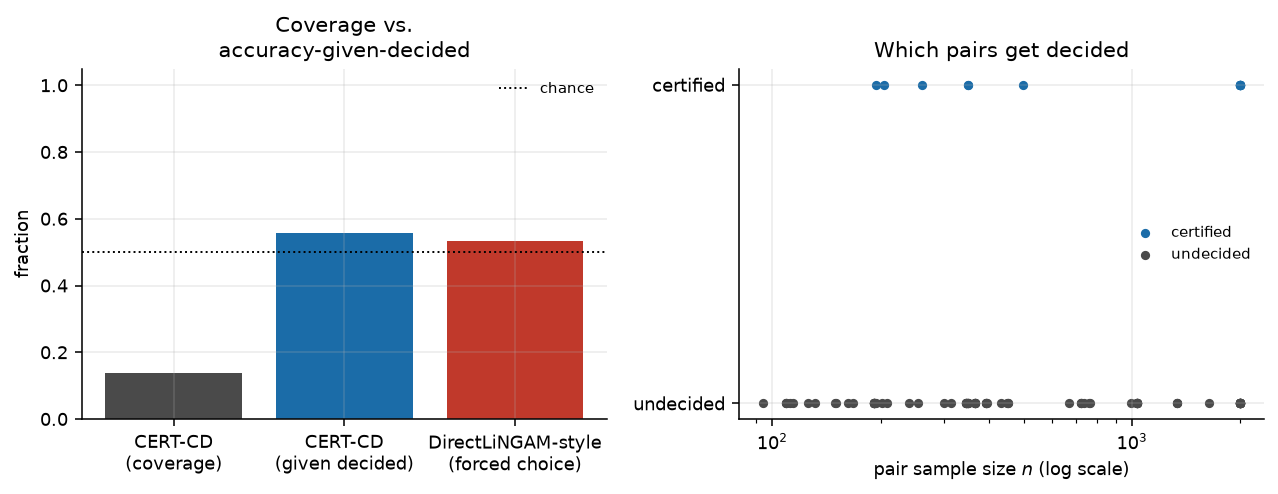
\includegraphics[width=0.95\textwidth]{figs/exp12_tuebingen_cep.png}
\caption{The direction certificate on $102$ Tübingen cause-effect pairs.
Left: coverage (fraction of pairs certified), weighted accuracy conditional on
certification, and the forced-choice comparison statistic's weighted
accuracy, against chance. Right: which pairs get decided, by sample
size.}\label{fig:exp12}
\end{figure}

\begin{figure}[t]
\centering
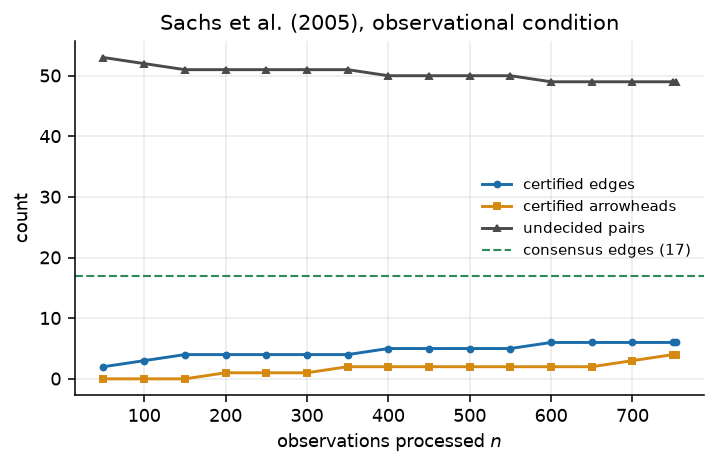
\includegraphics[width=0.75\textwidth]{figs/exp10_sachs.png}
\caption{CERT-CD on the Sachs observational sample. Certified edges accumulate
slowly and the undecided set stays large: at $n = 753$, $49$ of $55$ pairs
remain undecided.}\label{fig:exp10}
\end{figure}

\subsection{Where the certificates are void}\label{sec:exp-violations}
Placeholder.


\section{Discussion}\label{sec:discussion}

\subsection{What the output does not say}

The absence of an edge in a CERT-CD graph means \emph{undecided}. The
algorithm cannot report that an edge is missing, and a pair may remain
undecided indefinitely if adjacency-faithfulness fails for it---which is
exactly the situation in which a delete-on-non-rejection method returns a
confident wrong answer. This is the price of the rule. We regard stating it as
preferable to concealing it, but it is a real cost: on the Sachs data the
honest output is six certified edges and forty-nine shrugs, and a practitioner
who needs a complete graph will not get one from this method. The optional
fourth verdict of Section~\ref{sec:negligible} recovers part of the missing
information at the cost of naming a margin $\delta$, and we think that trade
is usually worth making in applications; we did not use it in the comparisons
above because the comparators assert absence outright and the comparison
should be with what they actually claim.

\subsection{Limitations}\label{sec:limitations}

We list these in what we take to be decreasing order of severity.

\begin{enumerate}
\item \emph{The direction certificate's family-wise bound is not delivered
  when its own premise fails, and the premise is correlated with
  faithfulness.} Section~\ref{sec:exp-main} measures a wrong-arrow rate of
  $0.080$ $([0.052, 0.120])$ against a budget of $0.05$ on instances violating
  $\delta$-strong faithfulness. Theorem~\ref{thm:main} is not contradicted---%
  its direction clause assumes the linear non-Gaussian model holds for the
  pair given its frozen block, and that assumption is what fails---but the
  practical reading of the theorem has to be adjusted: only the adjacency
  clause is robust to unfaithfulness. Freezing the conditioning block to all
  other variables rather than to the certified neighbours would decouple the
  two layers, at a cost in power we have not measured.

\item \emph{Misspecification of the direction certificate is not controlled
  more generally.} Proposition~\ref{prop:direction} requires the fitted
  supremum to dominate the likelihood at the true null parameter, which is
  guaranteed only when the noise lies in the fitted family.
  Section~\ref{sec:exp-sachs} shows this failing on real data,
  systematically and without any signal in the output. Bounding the gap---or
  replacing the generalised-Gaussian family with one whose supremum can be
  bounded under a nonparametric neighbourhood---is the most important open
  problem we leave.

\item \emph{Assumption~\ref{ass:sep} can fail, and fails silently.} It is more
  often satisfied than $\delta$-strong faithfulness
  (Table~\ref{tab:premises}), but ``more often'' is not ``always'', and
  Section~\ref{sec:exp-violations} shows that when it fails the family-wise
  bound is void rather than degraded. It is as unverifiable in practice as the
  assumption it replaces.

\item \emph{Causal sufficiency for the direction certificate.} The arrowhead
  null assumes no unobserved common cause of the pair.
  Section~\ref{sec:exp-violations} measures what latent confounding does; the
  answer is that arrowheads become unreliable well before adjacencies do.
  CERT-FCI (Section~\ref{sec:latent}) drops the direction certificate for this
  reason, and its FCI-rule orientations carry no family-wise guarantee.

\item \emph{The multiplicity layer is a union bound.}
  Section~\ref{sec:multiplicity} explains why nothing sharper is currently
  available for dependent pseudo e-values, and that a solution would improve
  every result here.

\item \emph{Scaling is unproven.} The direction layer refits per pair per
  batch and does not reduce to a sufficient statistic; experiments reach
  $d = 11$ on real data and $d = 7$ in simulation. Section~\ref{sec:complexity}
  identifies two straightforward optimisations we have not implemented, but we
  make no claim about behaviour at $d$ in the hundreds.

\item \emph{The FCI variant is incomplete.} It implements orientation rules
  R1--R4 and omits R5--R10, so its PAG is sound but not maximally informative.

\item \emph{Power is unquantified in theory.} We report certification rates
  empirically throughout, but we prove nothing about them. A power analysis
  under adjacency-faithfulness with a stated margin would be a natural
  companion result and we do not have one.
\end{enumerate}

\subsection{Outlook}

Three directions seem worth pursuing. The first is the multiplicity problem of
Section~\ref{sec:multiplicity}: family-wise control for dependent pseudo
e-values would be useful well beyond causal discovery. The second is replacing
the generalised-Gaussian direction likelihoods with a family admitting a
computable supremum under misspecification, which would close the gap that
Section~\ref{sec:exp-sachs} exposes; the reverse-regression characterisation
of \citet{ding2025gaussdetect} and the nonparametric route of
\citet{he2026sequential} both look promising. The third is interventional
data, where the certificate-only rule has an obvious analogue---an
intervention that changes a variable's distribution certifies an ancestral
relation by rejecting invariance---and where \citet{peters2016causal} already
provides the one-sided logic that Section~\ref{sec:exp-eicp} makes
anytime-valid.

\section{Conclusion}\label{sec:conclusion}

Constraint-based causal discovery deletes edges on non-rejection, and this
single design decision is the source of both its dependence on faithfulness
for finite-sample correctness and its inability to distinguish an established
absence from an unexamined pair. We asked what an algorithm looks like if it
refuses to do that: assert only by rejecting a null that is true whenever the
asserted feature is absent.

The answer is an algorithm that grows from the empty graph, reports undecided
pairs as undecided, and bounds by $\alpha$ the probability that any asserted
edge or arrowhead is ever wrong, uniformly over time and over the whole graph.
Adjacency is certified by an e-process for a union null, requiring the Markov
condition and a separator-size bound but no faithfulness. Orientation is
certified by sequential universal inference against the reversed
factorisation, escaping the Markov equivalence class and abstaining
automatically under Gaussianity. What the design costs is power, and we have
tried to report that cost as prominently as the guarantee---in the power
curves of Section~\ref{sec:exp-calibration}, the undecided fractions of
Section~\ref{sec:exp-main}, and the six-edges-out-of-fifty-five of
Section~\ref{sec:exp-sachs}.

The Sachs experiment also delivers the paper's own counterexample. Where the
certifying null rests on the Markov condition alone, the method behaves as
advertised on real data. Where it rests on a parametric functional model, the
method is confidently and systematically wrong, with nothing in its output to
say so. A certificate is only ever as good as the null it certifies against,
and we think making that dependence visible---rather than absorbing it into an
assumption stated once and not revisited---is the more useful contribution.

\backmatter

\section*{Statements and Declarations}\label{sec:declarations}

\paragraph{Competing interests.} The author declares no competing interests.

\paragraph{Funding.} This research received no specific grant from any funding
agency in the public, commercial, or not-for-profit sectors.

\paragraph{Ethics approval.} Not applicable. The study involves no human
participants or animals. The protein-signalling data analysed in
Section~\ref{sec:exp-sachs} are publicly available and were published by
\citet{sachs2005causal}.

\paragraph{Data and code availability.}\label{sec:availability} All
simulation code, experiment scripts, random seeds and figure-generating
scripts are available at
\url{https://github.com/vinhqdang/SPRINT-CD}. The protein-signalling data of
\citet{sachs2005causal} are redistributed with the \texttt{bnlearn} package
\citep{scutari2010learning} and are downloaded by the experiment script rather
than included in the repository. The Tübingen cause-effect pairs of
Section~\ref{sec:exp-tuebingen} are likewise downloaded on first use from
\url{https://webdav.tuebingen.mpg.de/cause-effect/} and are not redistributed.

\paragraph{Author contributions.} The author is solely responsible for all
aspects of this work.

\paragraph{Use of generative AI in the preparation of this manuscript.} A
large language model was used in support of writing this manuscript. The
author verified and modified the resulting content and takes full
responsibility for the manuscript in its entirety, including its claims,
derivations, experiments and references.
